\label{dist_rel_generalisation}

\par Les modèles décrits dans cette section appartiennent à la seconde classe (\ref{dist_rel_classes_explication}). Leur objectif est de valider les paramètres et les entrées des modèles de la première classe, et de généraliser la méthode à plusieurs liaisons différentes. Pour cela, nous préparons des jeux de données de grandes tailles, et nous entraînons les modèles sur 300 époques, pour les liaisons carbone-carbone, carbone-hydrogène et oxygène-hydrogène. Les tailles des jeux de données pour chacun des modèles sont données dans le tableau \ref{t_tailles_dist_rel_xy}. Si seulement une partie des molécules est explorée pour générer les jeux de données concernant les liaisons carbone-carbone et carbone-hydrogène du fait de leur grande représentation dans les données, toutes les molécules sont explorées pour générer les exemples concernant les liaisons oxygène-hydrogène, qui sont moins nombreuses dans les molécules de notre jeu de données (\ref{donnees_bases}).
\par Notons que les modèles \emph{DIST\_REL\_C} et \emph{DIST\_REL\_CC} prédisent les mêmes longueurs de liaisons (carbone-carbone), la différence entre les deux étant la taille des jeux de données utilisés et la durée d'entraînement.

\begin{table}
	\centering
		\begin{tabular}{|l|l|l|l|}
			\hline
			\textbf{Jeu} & \textbf{Modèles \emph{DIST\_REL\_CC}} & \textbf{Modèles \emph{DIST\_REL\_CH}} & \textbf{Modèles \emph{DIST\_REL\_OH}} \\ \hline
			Entraînement & 5541305 & 3636608 & 1293551 \\ \hline
			Test & 1106823 & 1158251 & 143588 \\ \hline
		\end{tabular}

	\caption{Tailles des jeux de données des modèles \emph{DIST\_REL\_XY}}
	\label{t_tailles_dist_rel_xy}
\end{table}

Les paramètres d'entraînement communs utilisés par tous les modèles \emph{DIST\_REL\_XY} sont donnés dans la tableau \ref{tparams_dist_rel_xy}.

\begin{table}
	\centering
	\begin{tabular}{|l|l|}
		\hline
		\textbf{Paramètre} & \textbf{Valeur} \\ \hline
		Taille de lot (\emph{batch size}) & 10000 \\ \hline
		Epsilon (Adam) & 0.001 \\ \hline
		Initialisation des poids (\emph{stddev\_init}) & 0.001 \\ \hline
		Fonction d'activation couches cachées & elu \\ \hline
		Fonction d'activation couche de sortie & linéaire \\ \hline
		Abandon (\emph{dropout}) & 0.98 \\ \hline
		Dégradation des coefficients (\emph{weight decay}) & 0.001 \\ \hline
	\end{tabular}

	\caption{Paramètres d'entraînement des modèles \emph{DIST\_REL\_XY}}
	\label{tparams_dist_rel_xy}
\end{table}

\subsection{Modèles naïfs}

\label{dist_rel_xy_naif}

Les trois modèles naïfs sont entraînés avec les mêmes paramètres et le même traitement des données d'entrée que leur modèle équivalent de la première classe (\ref{dist_rel_c_naif}), c'est à dire qu'aucune restriction au voisinage le plus proche de la liaison n'est appliquée, et qu'aucune fonction n'est appliquée aux distances.

\subsubsection{Analyse statistique des erreurs}
\par Dans le tableau \ref{t_stats_dist_rel_xy_01}, nous présentons les valeurs des différentes métriques permettant d'évaluer les erreurs pour les modèles prédisant chaque type de liaison. Afin de comparer les performances du modèle prédisant les longueurs de liaisons carbone-carbone avec le modèle de la première classe équivalent, nous rappelons également la valeur des métriques du modèle \emph{DIST\_REL\_C\_01}.
\par L'entraînement sur un nombre plus élevé d'exemples fait apparaître un gain non négligeable pour la prédiction de longueurs de liaisons entre des atomes de carbone. La moyenne passe en effet en dessous de la barre cible de 1 pm. L'écart-type est cependant toujours au dessus du pm, même si sa valeur est peu interprétable du fait de la distribution non gaussienne des erreurs.
\par La prédiction des autres types de liaisons montre de très bons résultats, la plupart des métriques étant à des valeurs proches du dixième de picomètre. Les erreurs maximales ont toutefois des valeurs relativement élevées, notamment dans le cas de la prédiction des liaisons carbone-hydrogène.

\begin{table}
	\centering
	\begin{tabular}{|l|r|r|r|r|}
		\hline
		\textbf{Métrique}& \textbf{\emph{D\_REL\_C\_01}} &\textbf{\emph{D\_REL\_CC\_01}} & \textbf{\emph{D\_REL\_CH\_01}} & \textbf{\emph{D\_REL\_OH\_01}}\\ \hline
		Moyenne & 1,3301 & 0,8334 & 0,1753 & 0,1947\\ \hline
		Médiane & 0,6881 & 0,4604 & 0,1132 & 0,1153\\ \hline
		Écart-type & 1,9810 & 1,2066 & 0,1961 & 0,2519 \\ \hline
		Minimum & 0,0000 & 0,0000 & 0.0000 & 0.0000\\ \hline
		Maximum & 28,7268 & 30,1138 & 22,1473 & 7,2530\\ \hline
		Erreur rel. & 0,9126\% & 0,5709\% & 0,1599\% & 0.1986\%\\ \hline
	\end{tabular}
	
	\caption{Analyse statistique des erreurs des modèles (en pm)}
	\label{t_stats_dist_rel_xy_01}
\end{table}

\subsubsection{Représentation graphique des résultats}

\par La distribution des erreurs des modèles prédisant les longueurs de liaisons entre les atomes de carbone et d'hydrogène et entre les atomes d'hydrogène et d'oxygène montre que les plus grosses erreurs sont marginales en représentation (figures \ref{fdistrib_err_dist_rel_ch_01} et \ref{fdistrib_err_dist_rel_oh_01}). \\


\begin{figure}
	\centering
	
	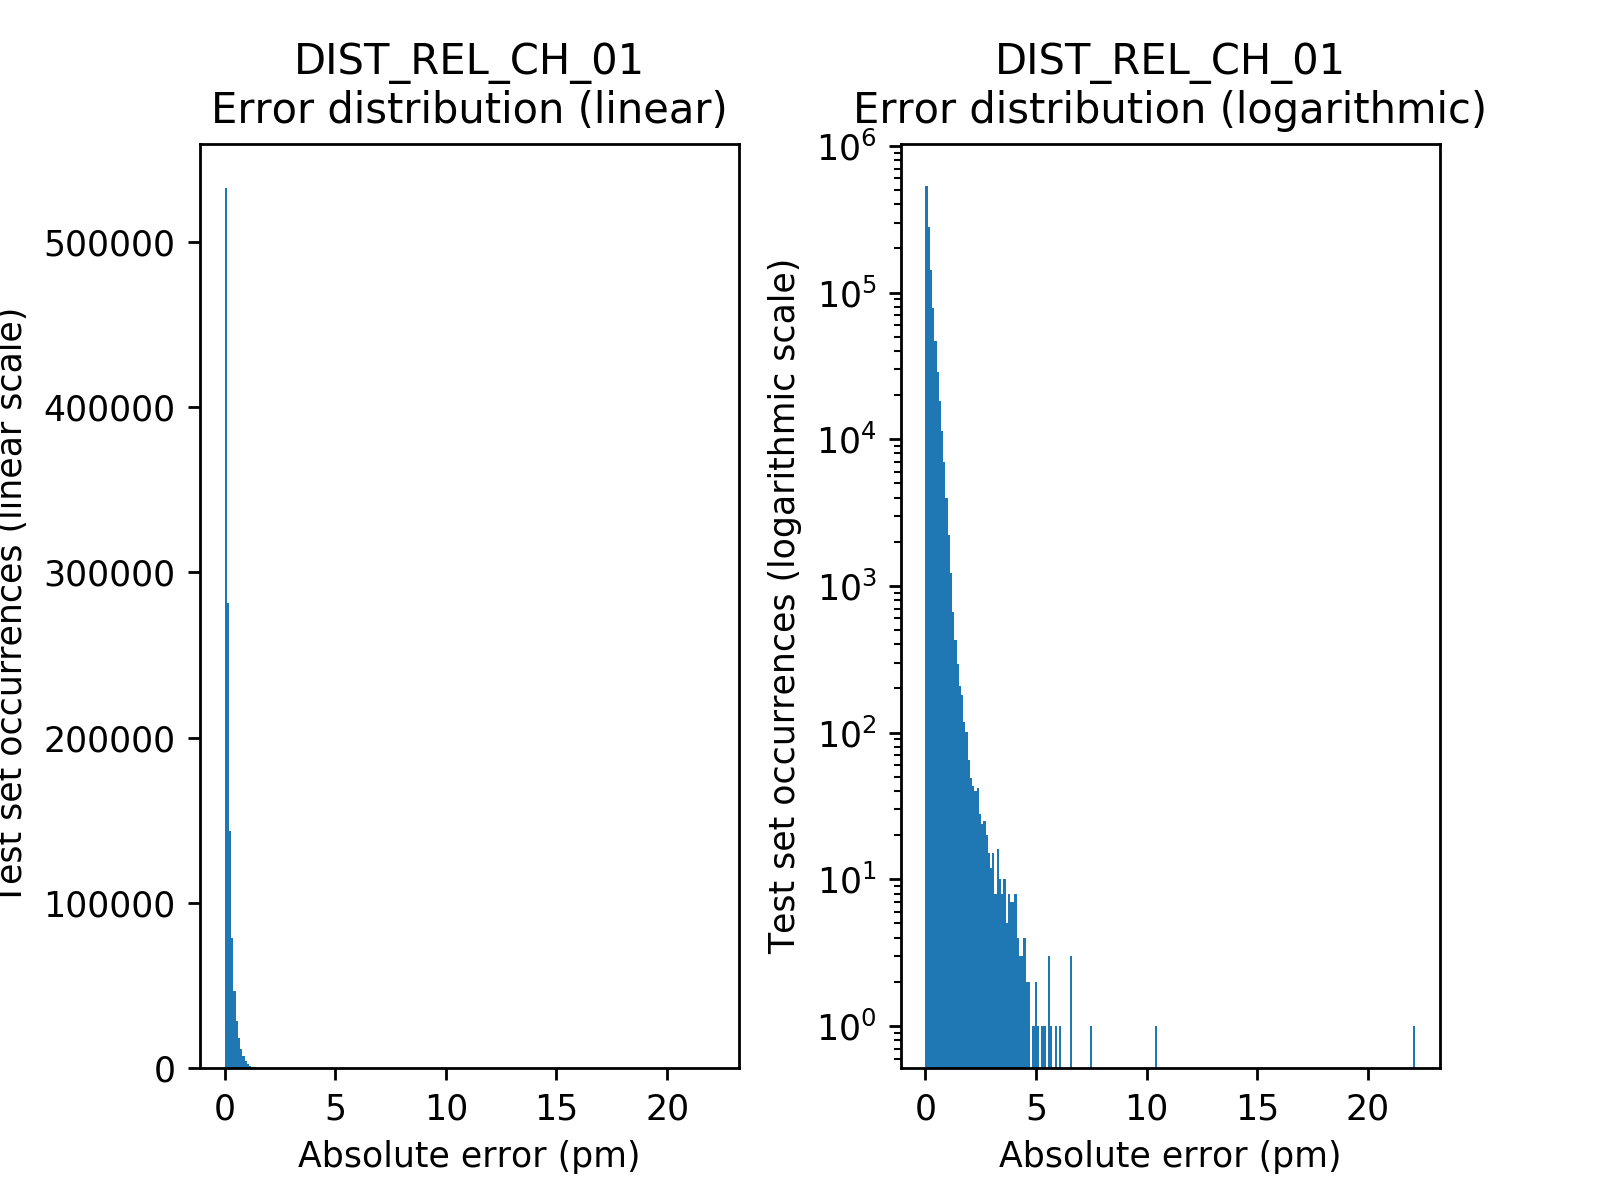
\includegraphics[scale=0.7]{../figures/DIST_REL_CH_01/DIST_REL_CH_01_distrib_rmse_val.png}	
	
	\caption{Distribution des erreurs du modèle \emph{DIST\_REL\_CH\_01}}
	\label{fdistrib_err_dist_rel_ch_01}

\end{figure}
\begin{figure}
	\centering
	
	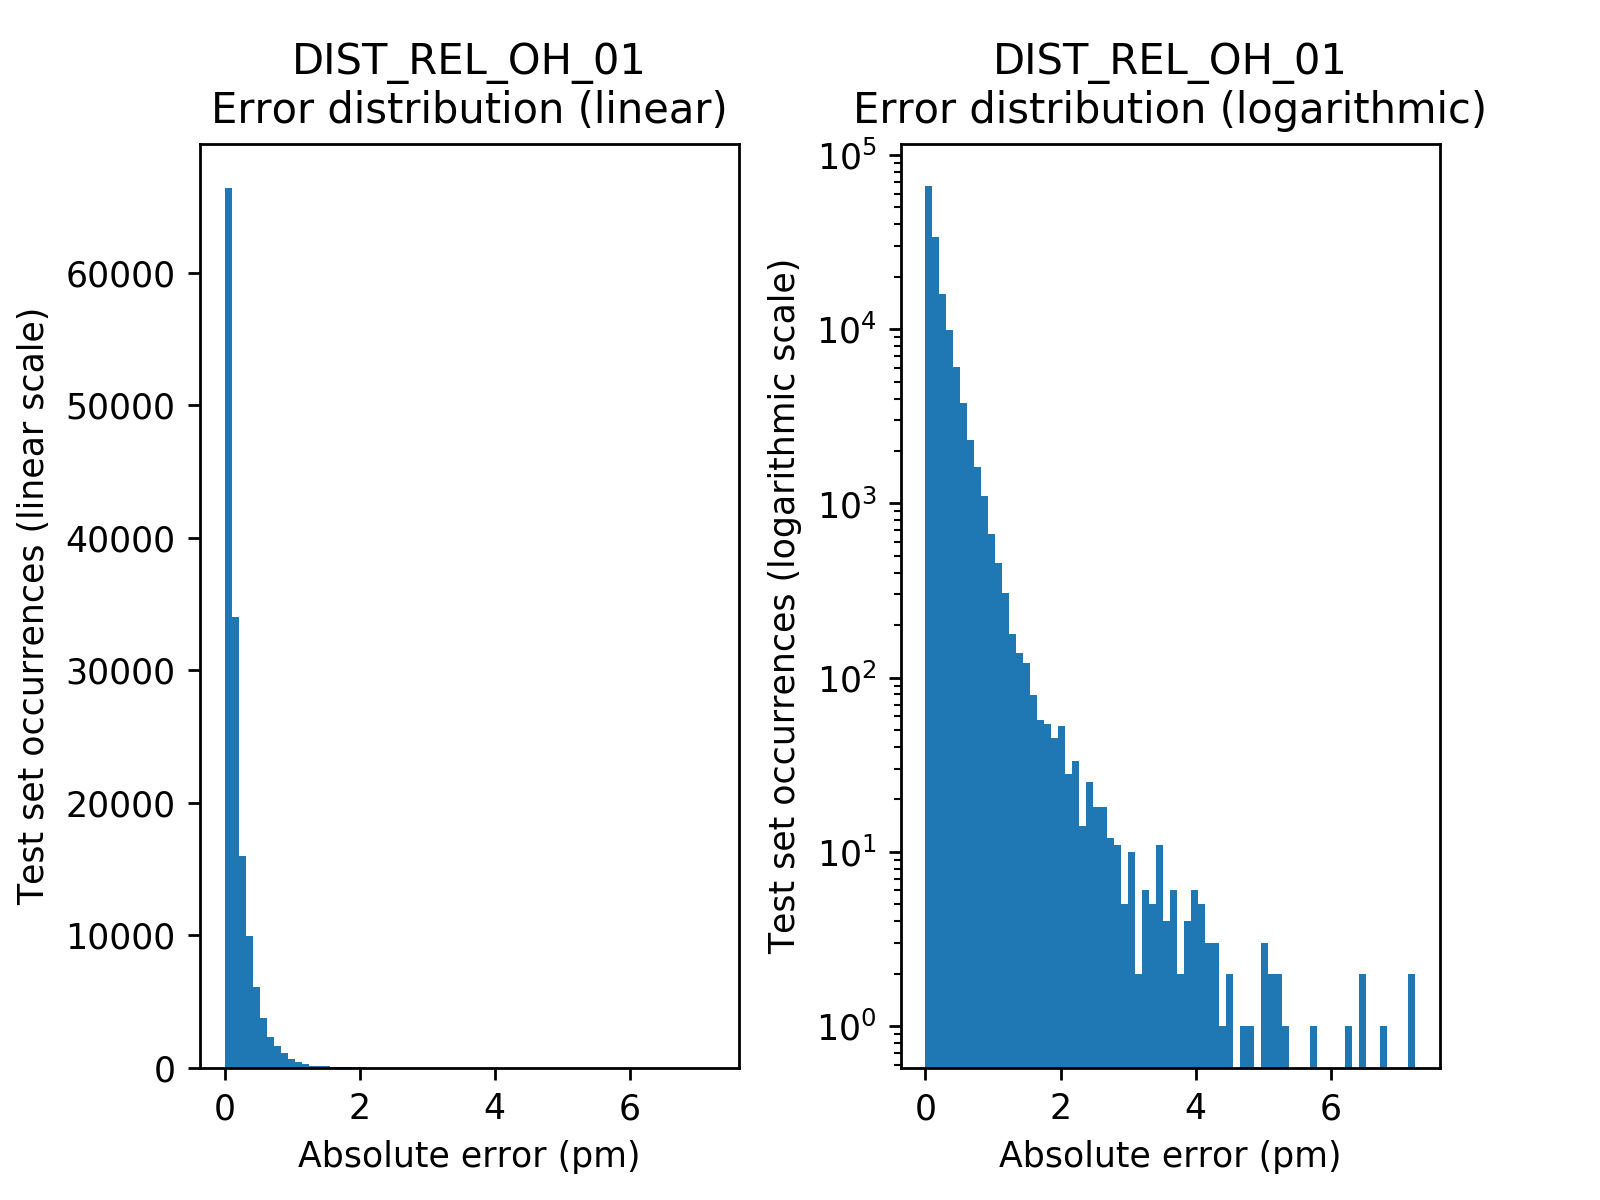
\includegraphics[scale=0.7]{../figures/DIST_REL_OH_01/DIST_REL_OH_01_distrib_rmse_val.png}	
	
	\caption{Distribution des erreurs du modèle \emph{DIST\_REL\_OH\_01}}
	\label{fdistrib_err_dist_rel_oh_01}

\end{figure}

\par La représentation graphique des erreurs relatives (figure \ref{fdistrib_err_rel_dist_rel_oh_01}) et des prédictions en fonction des cibles (figure \ref{fpreds_targets_dist_rel_oh_01}) montre un phénomène intéressant pour le modèle prédisant les longueurs de liaisons entre les atomes d'oxygène et d'hydrogène. La représentation des longueurs de liaisons OH chutant brusquement en deçà de 97 pm, le modèle s'adapte à cette particularité en ne prédisant jamais des valeurs inférieures à 97 pm.

\begin{figure}
	\centering
	
	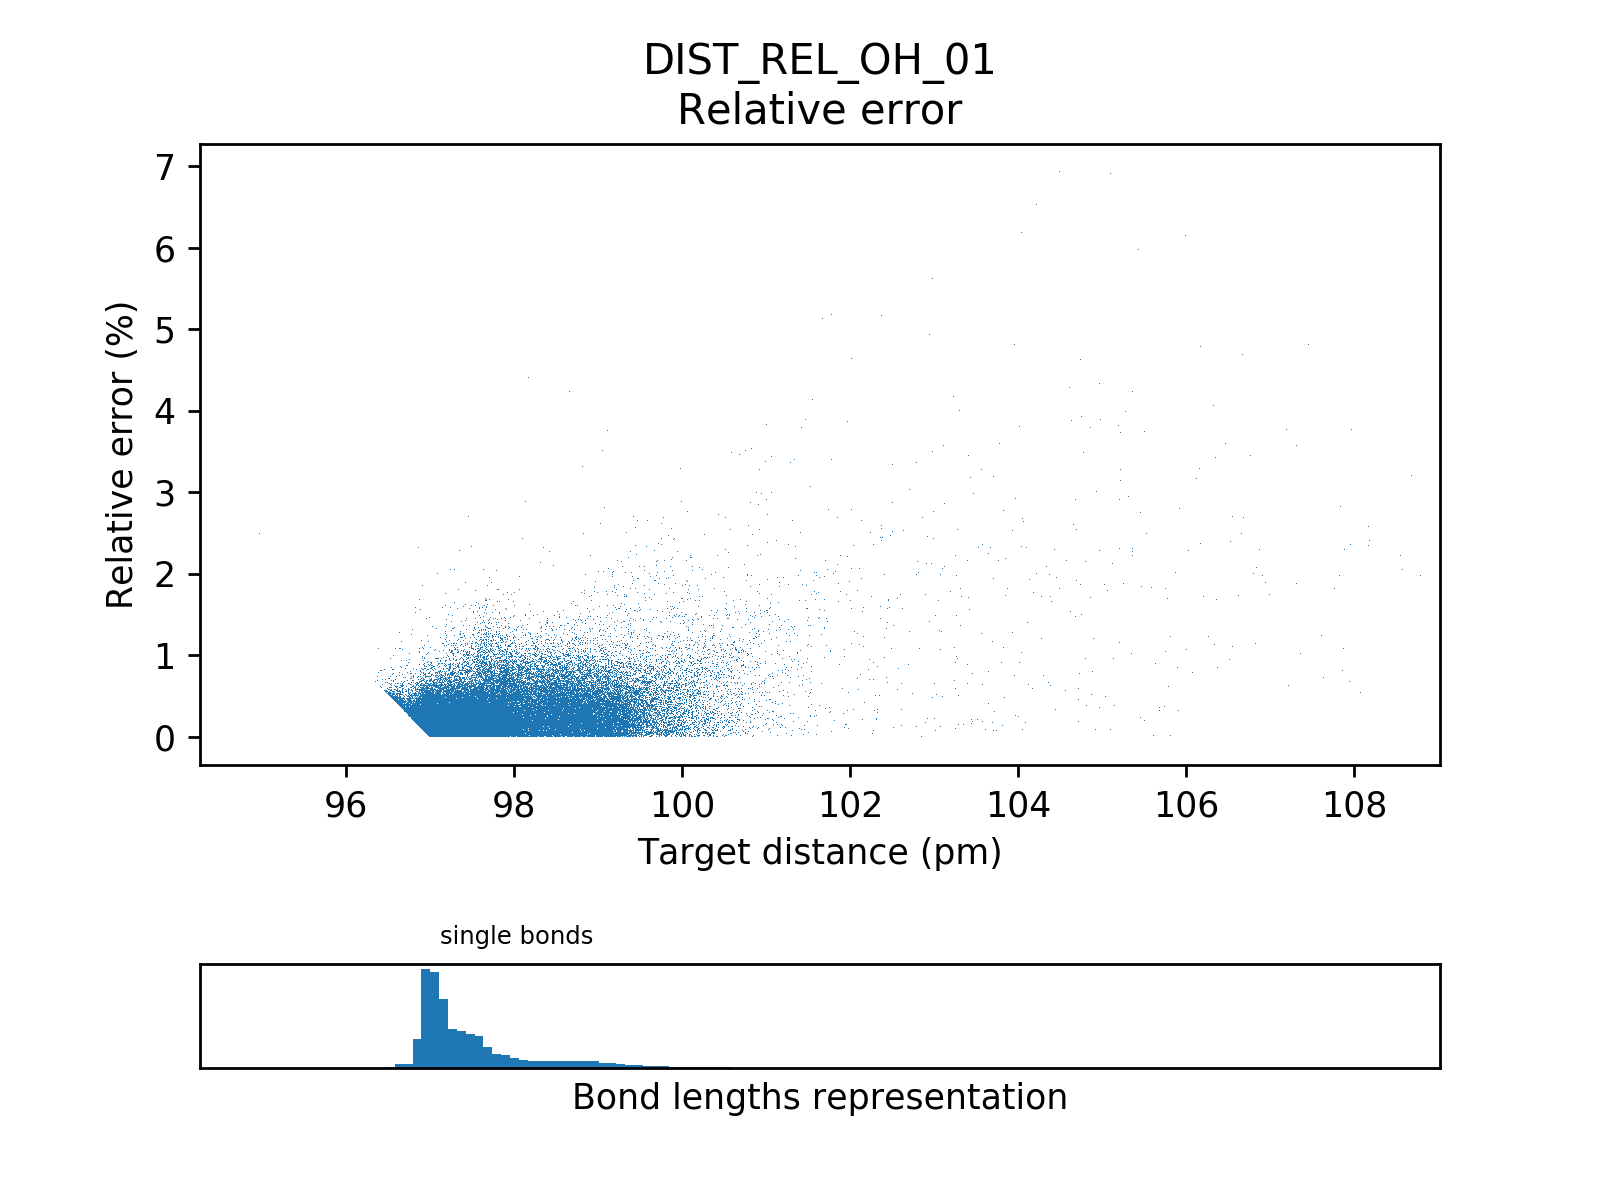
\includegraphics[scale=0.7]{../figures/DIST_REL_OH_01/DIST_REL_OH_01_distrib_rmse_dist.png}	
	
	\caption{Erreur en fonction des cibles pour le modèle \emph{DIST\_REL\_OH\_01}}
	\label{fdistrib_err_rel_dist_rel_oh_01}
	\end{figure}
	
\begin{figure}
	\centering
	
	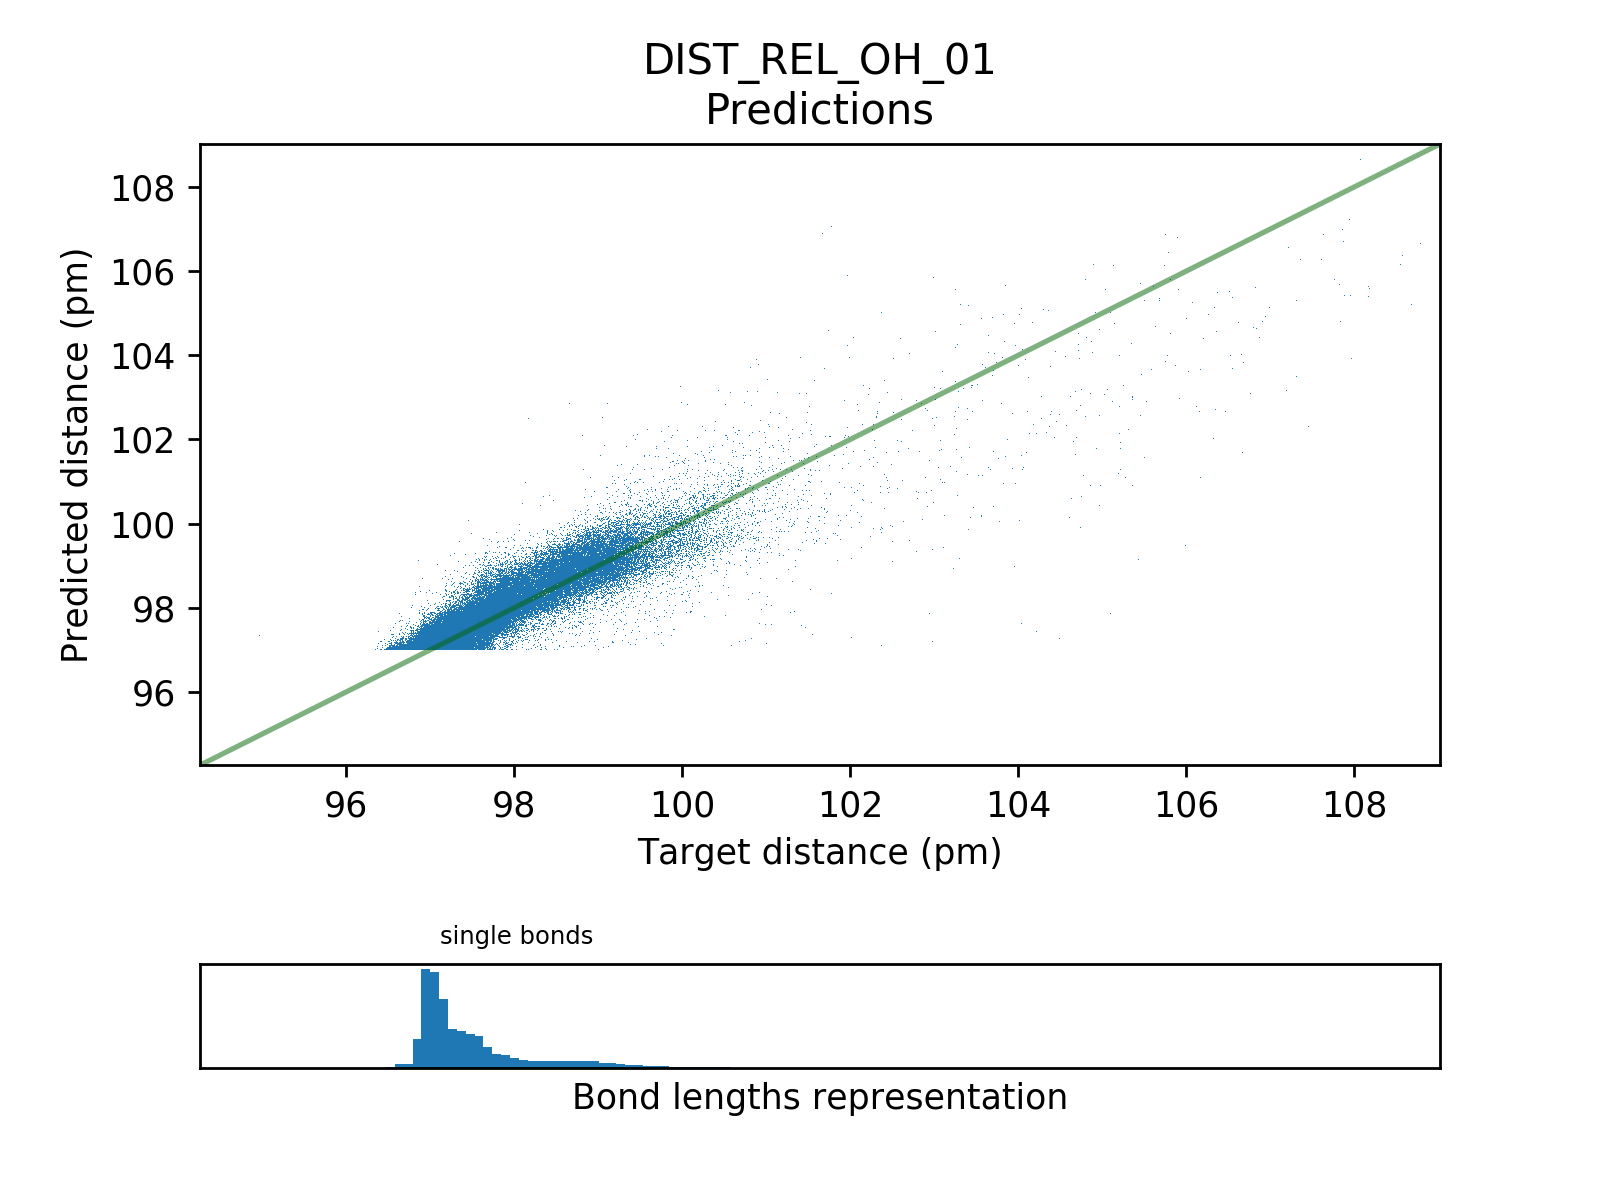
\includegraphics[scale=0.7]{../figures/DIST_REL_OH_01/DIST_REL_OH_01_preds_targets.png}	
	
	\caption{Prédictions en fonction des cibles pour le modèle \emph{DIST\_REL\_OH\_01}}
	\label{fpreds_targets_dist_rel_oh_01}

\end{figure}

\par Enfin, la représentation graphique des erreurs relatives (figure \ref{fdistrib_err_rel_dist_rel_ch_01}) et des prédictions (figure \ref{fpreds_targets_dist_rel_ch_01}) du modèle prédisant les longueurs de liaison carbone-hydrogène montre que les très bons résultats du modèle s'expliquent en partie par la faible dispersion des longueurs cibles.\\
Les représentations graphiques concernant le modèle prédisant les liaisons carbone-carbone étant très semblables à celles du modèle \emph{DIST\_REL\_C\_01}, elles sont uniquement visibles en annexe \ref{annexes_plot_dist_rel_xy}.

\begin{figure}
	\centering
	
	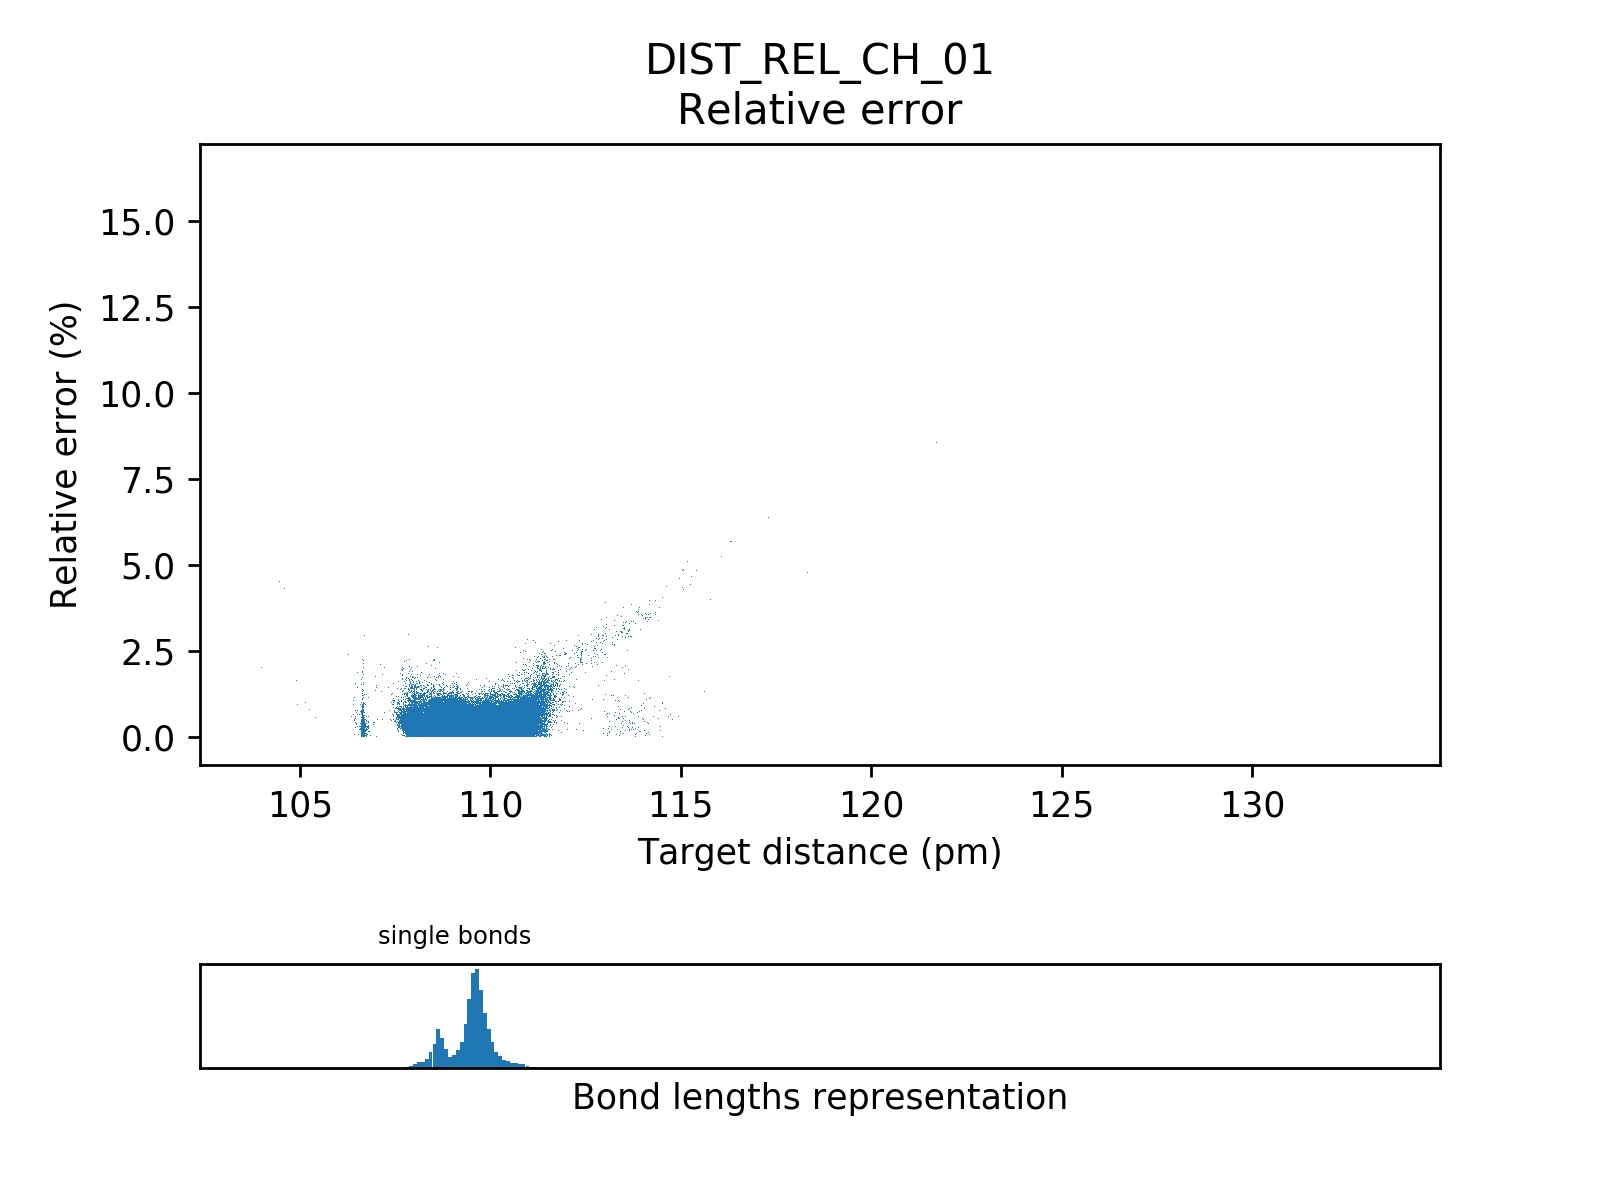
\includegraphics[scale=0.7]{../figures/DIST_REL_CH_01/DIST_REL_CH_01_distrib_rmse_dist.png}	
	
	\caption{Erreur en fonction des cibles pour le modèle \emph{DIST\_REL\_CH\_01}}
	\label{fdistrib_err_rel_dist_rel_ch_01}
	\end{figure}
	
\begin{figure}
	\centering
	
	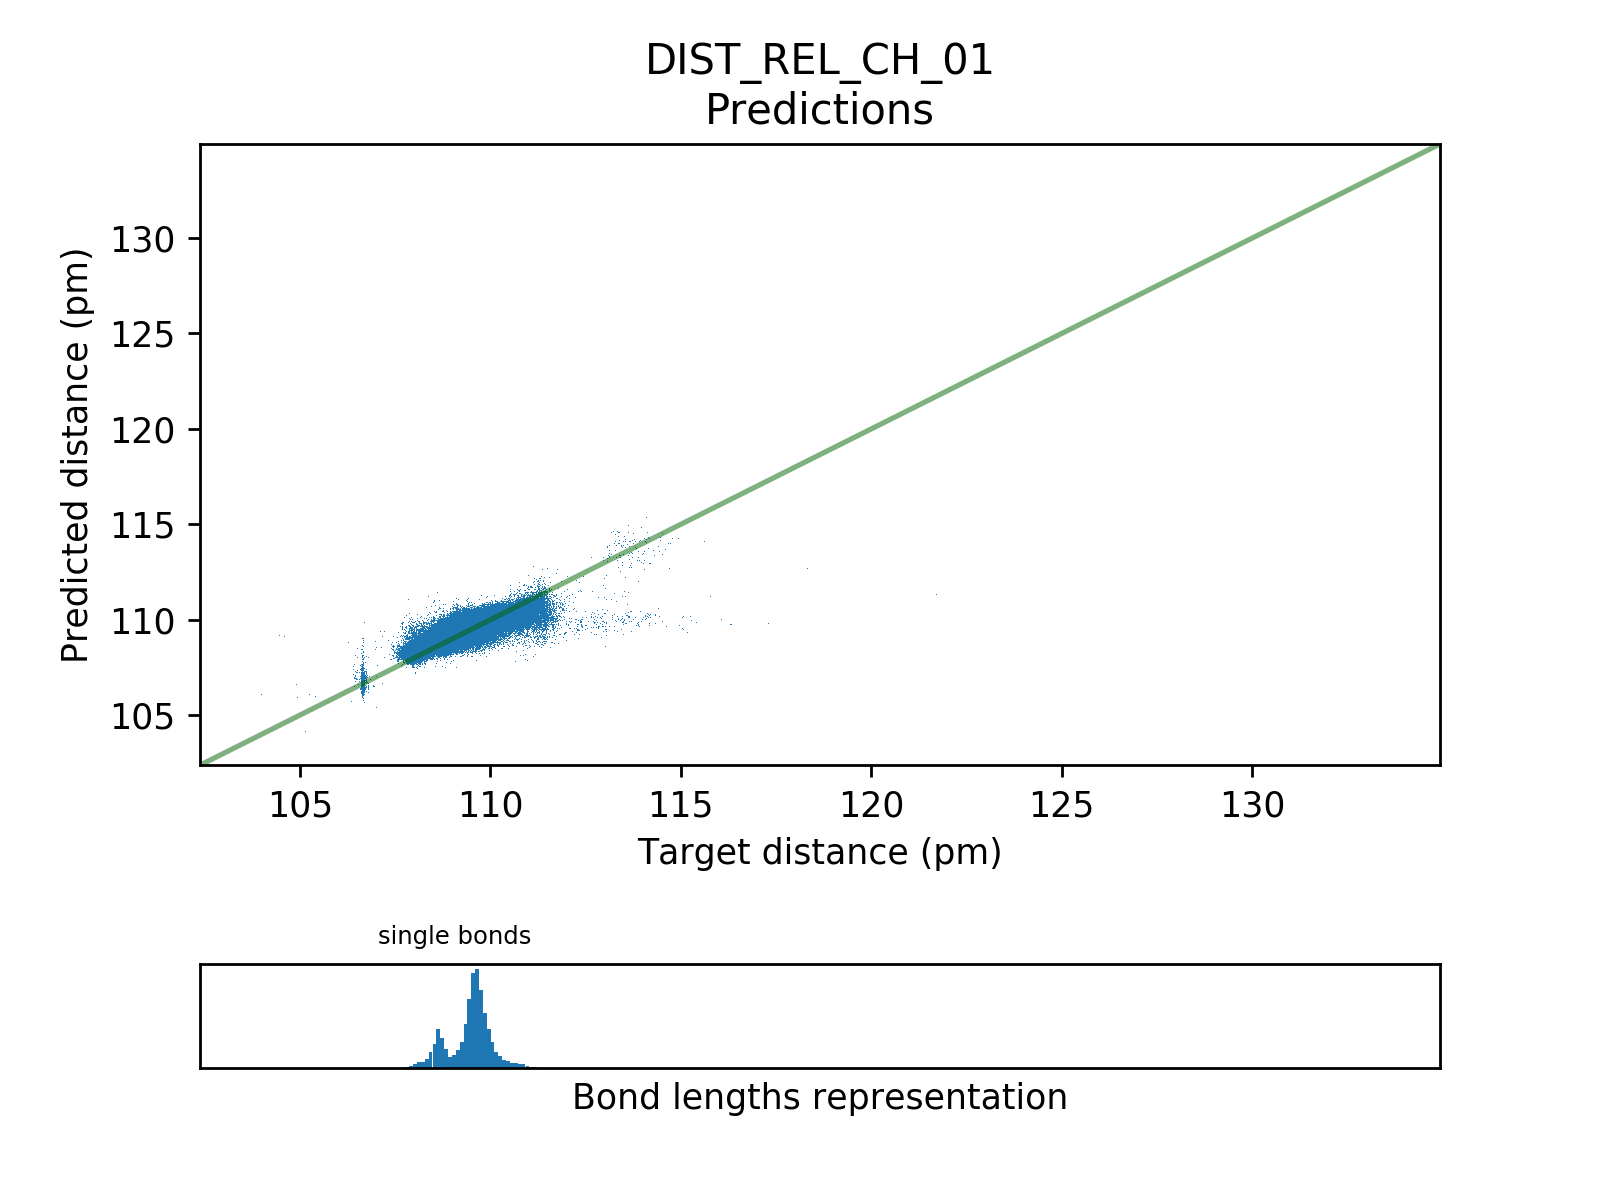
\includegraphics[scale=0.7]{../figures/DIST_REL_CH_01/DIST_REL_CH_01_preds_targets.png}	
	
	\caption{Prédictions en fonction des cibles pour le modèle \emph{DIST\_REL\_CH\_01}}
	\label{fpreds_targets_dist_rel_ch_01}

\end{figure}

\subsection{Restriction au voisinage le plus proche}

\label{dist_rel_xy_restrict}

\par Les modèles décrits dans cette partie sont les modèles de la seconde classe équivalents aux modèles décrits en \ref{dist_rel_c_restriction}.

\subsubsection{Analyse statistique des erreurs}
\par Le tableau \ref{tstats_dist_rel_xy_02} donne les valeurs des différentes métriques évaluant les erreurs des modèles. Comme attendu, la restriction aux atomes au plus proche voisinage améliore en général les performances des modèles, notamment dans le cas du modèle prédisant les longueurs de liaisons entre des atomes de carbone. Les prédictions concernant les longueurs de liaisons entre des atomes d'hydrogène et d'oxygène sont également améliorées d'un facteur moindre. Toutefois, les prédictions des longueurs de liaisons entre des atomes de carbone et d'hydrogène sont impactées négativement par cette nouvelle approche, même si l'erreur maximale est diminuée d'un facteur trois.


\begin{table}
	\centering
	\begin{tabular}{|l|r|r|r|}
		\hline
		\textbf{Métrique}& \textbf{\emph{DIST\_REL\_CC\_02}} & \textbf{\emph{DIST\_REL\_CH\_02}} & \textbf{\emph{DIST\_REL\_OH\_02}}\\ \hline
		Moyenne & 0,3416 & 0,2390 & 0,1519\\ \hline
		Médiane &  0.2667 & 0.2010 &  0,1044\\ \hline
		Écart-type & 0,3373 & 0,1884 & 0,1648 \\ \hline
		Minimum & 0,0000 & 0,0000 & 0.0000\\ \hline
		Maximum & 26.2167 & 6,2905 & 4,7264 \\ \hline
		Erreur rel. & 0,2295\% & 0,2184\% & 0,1552\%\\ \hline
	\end{tabular}
	
	\caption{Analyse statistique des erreurs des modèles (en pm)}
	\label{tstats_dist_rel_xy_02}
\end{table}

\subsubsection{Analyse graphique des résultats}

\par Les représentations graphiques des erreurs (figures \ref{fdistrib_err_dist_rel_cc_02} et \ref{fdistrib_err_rel_dist_rel_cc_02}) et des prédictions (figure \ref{fpreds_targets_dist_rel_cc_02}) du modèle prédisant les longueurs de liaisons entre des atomes de carbone font nettement apparaître la diminution des erreurs importantes et la continuité des prédictions entre les différents types de liaisons.


\begin{figure}
	\centering
	
	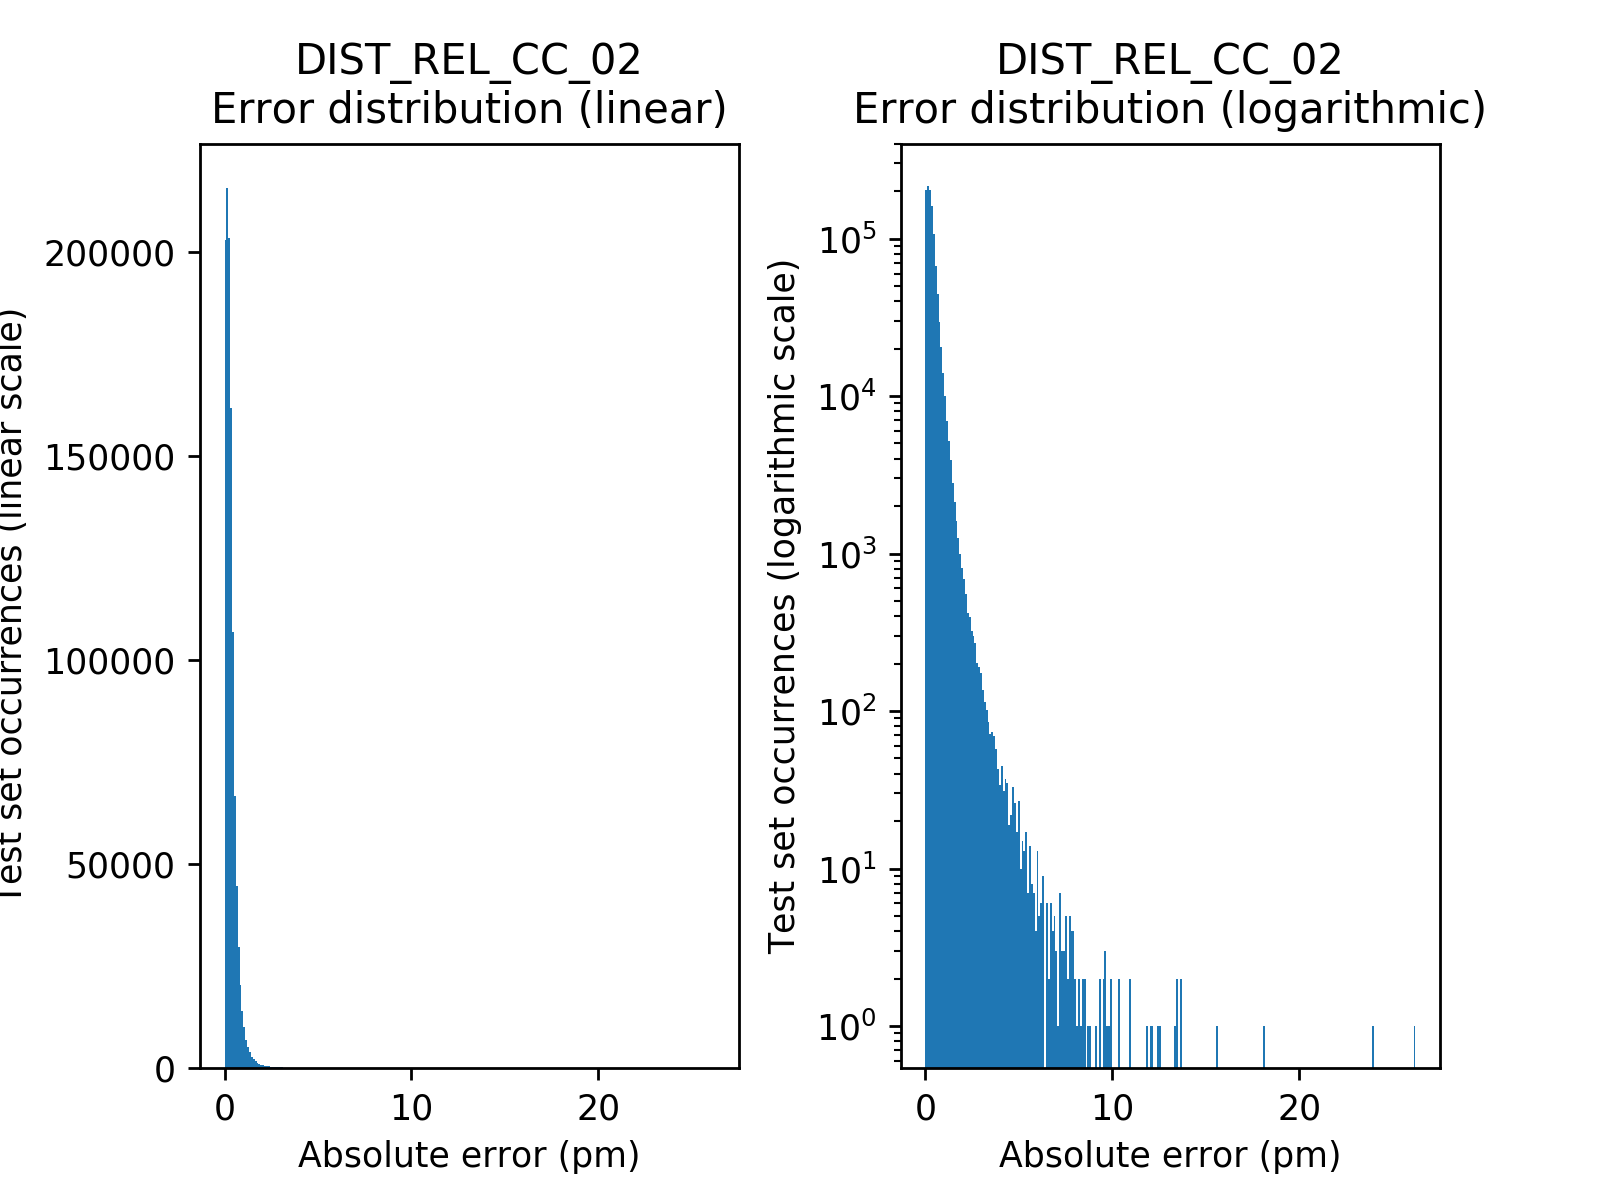
\includegraphics[scale=0.8]{../figures/DIST_REL_CC_02/DIST_REL_CC_02_distrib_rmse_val.png}	
	
	\caption{Distribution des erreurs du modèle \emph{DIST\_REL\_CC\_02}}
	\label{fdistrib_err_dist_rel_cc_02}
\end{figure}
\begin{figure}
	\centering
	
	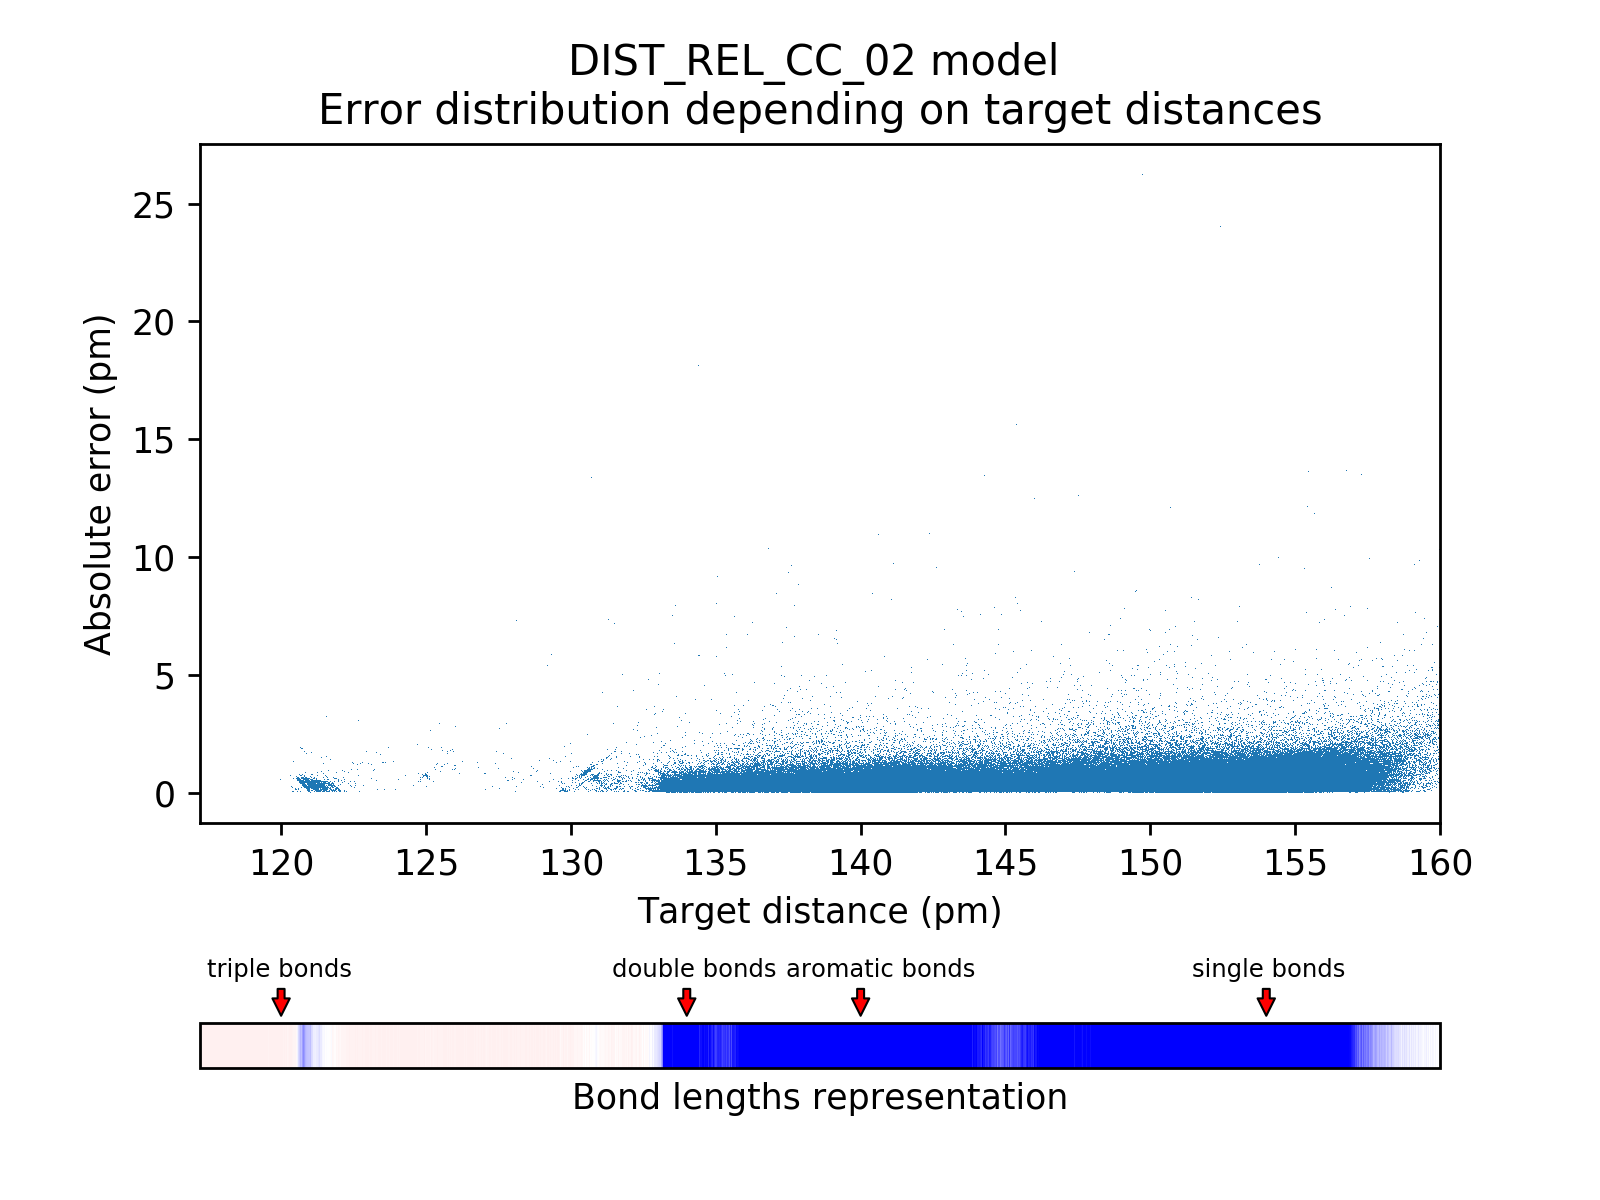
\includegraphics[scale=0.8]{../figures/DIST_REL_CC_02/DIST_REL_CC_02_distrib_rmse_dist.png}	
	
	\caption{Erreur en fonction des cibles pour le modèle \emph{DIST\_REL\_CC\_02}}
		\label{fdistrib_err_rel_dist_rel_cc_02}

	\end{figure}

\begin{figure}
	\centering
	
	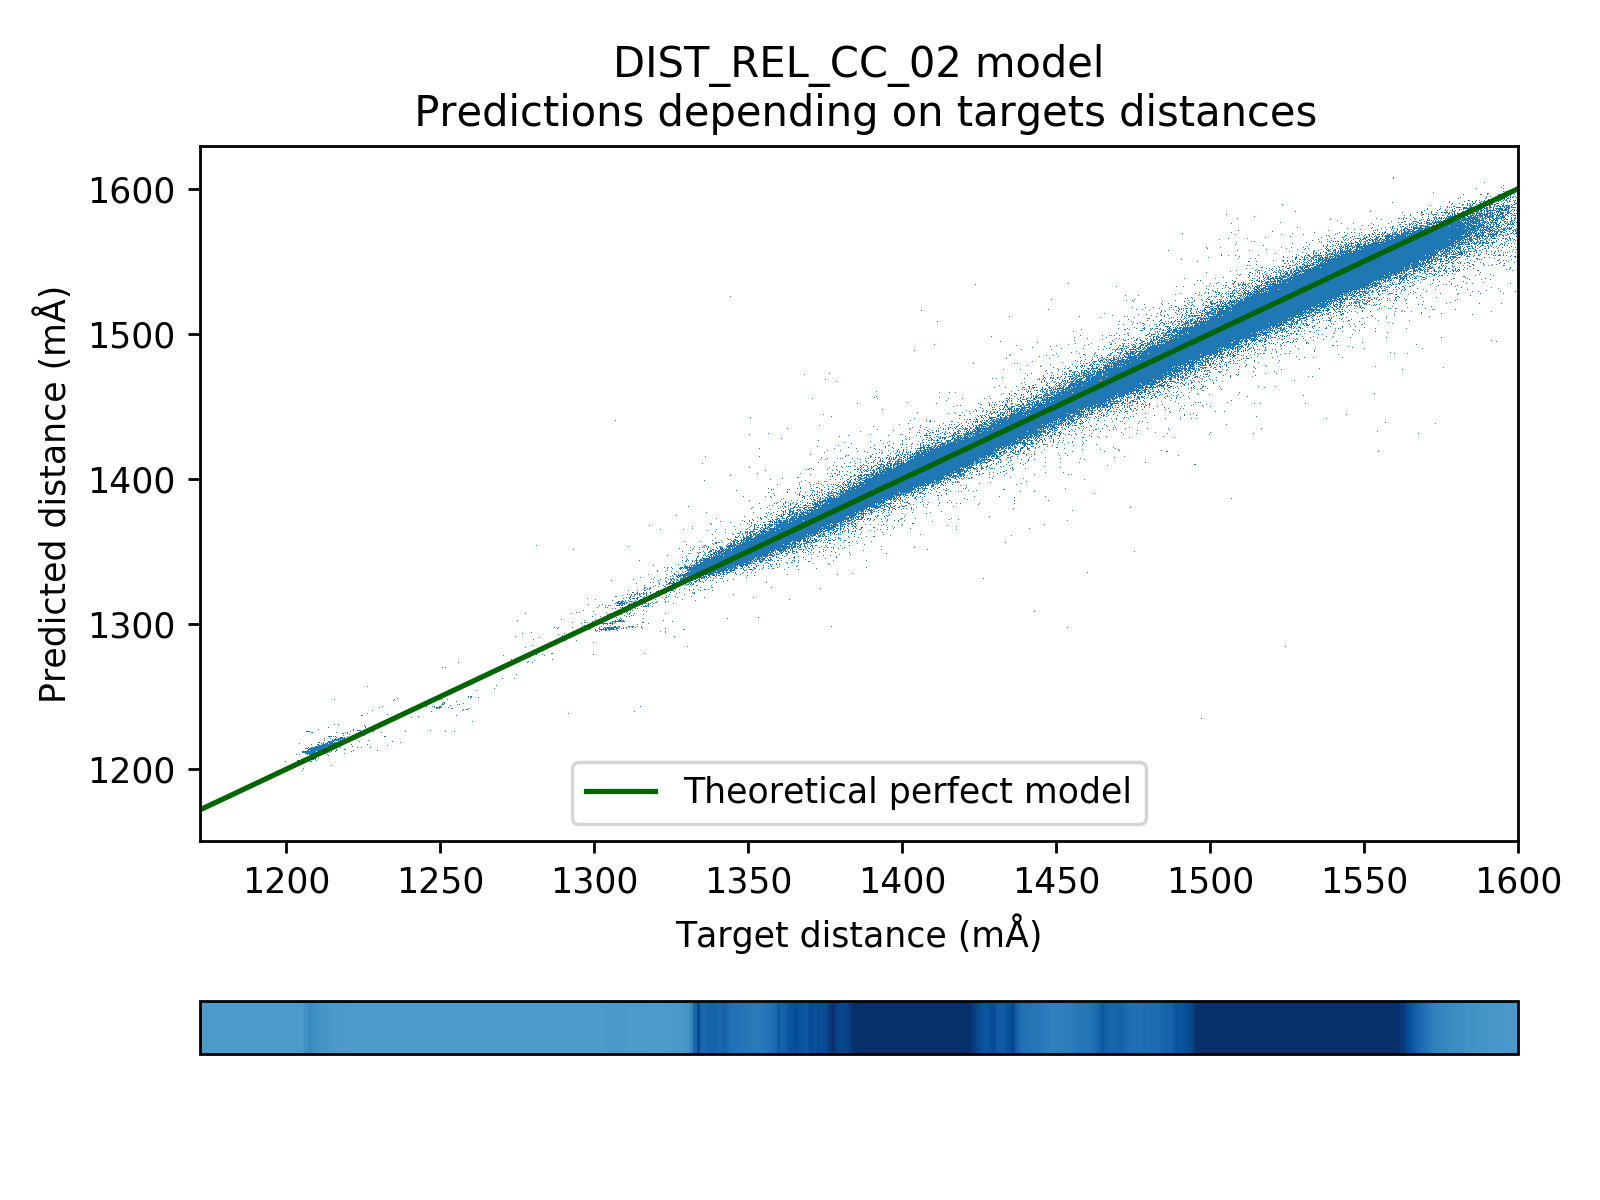
\includegraphics[scale=0.8]{../figures/DIST_REL_CC_02/DIST_REL_CC_02_preds_targets.png}	
	
	\caption{Prédictions en fonction des cibles pour le modèle \emph{DIST\_REL\_CC\_02}}
	\label{fpreds_targets_dist_rel_cc_02}
	
\end{figure}

\par La représentation graphique des erreurs et prédictions des deux autres modèles fait apparaître la légère amélioration des prédictions du modèle prédisant les longueurs de liaisons entre les atomes d'oxygène et d'hydrogène, et la baisse de performances du modèle prédisant les longueurs de liaisons entre les atomes de carbone et d'hydrogène. Elles sont disponibles en annexe \ref{annexes_plot_dist_rel_xy}.
	
\subsection{Application de fonctions aux distances}

\label{dist_rel_xy_fun}


\label{dist_rel_generalisation_fonctions}

\par L'application de fonctions aux distances en entrée des modèles (\ref{dist_rel_c_fun}) donne des résultats mitigés lorsqu'on tente de généraliser la méthode à plusieurs liaisons différentes sur des jeux d'entraînement plus grands. Les tableaux \ref{tstats_dist_rel_xy_03} et \ref{tstats_dist_rel_xy_04} présentent les valeurs des métriques évaluant les erreurs des modèles lorsqu'on applique la fonction inverse et carré de l'inverse aux distances en entrée. Les représentations graphiques des résultats sont disponibles en annexe \ref{annexes_plot_dist_rel_xy}. Notons que contrairement aux modèles de la première classe, le modèle \emph{DIST\_REL\_X\_03} (resp. \emph{DIST\_REL\_X\_04}) correspond à l'application de la fonction carré de l'inverse (resp. fonction inverse). Cela est dû au fait que seule la fonction carré de l'inverse devait être initialement appliquée, au vu de ses meilleurs résultats sur le modèle de la première classe. Ses résultats mitigés lors de la généralisation à d'autres liaisons nous ont cependant poussé à tester également la fonction inverse.\\
Notons enfin que les modèles décrits ici appliquent la restriction aux atomes au voisinage le plus proche (\ref{repr_locale_liaisons_cov_restrict}), avec une valeur $\epsilon$ de 200 pm.\\

\begin{table}
	\centering
	\begin{tabular}{|l|r|r|r|}
		\hline
		\textbf{Métrique}& \textbf{\emph{DIST\_REL\_CC\_03}} & \textbf{\emph{DIST\_REL\_CH\_03}} & \textbf{\emph{DIST\_REL\_OH\_03}}\\ \hline
		Moyenne & 0,4508 & 0,1634 & 0,2107\\ \hline
		Médiane &  0,3290 & 0,1206 &  0,1832\\ \hline
		Écart-type & 0,4582 & 0,1591 & 0,1742 \\ \hline
		Minimum & 0,0000 & 0,0000 & 0,0000\\ \hline
		Maximum & 16,6302 & 6.1820 & 7,0743 \\ \hline
		Erreur rel. & 0,3017\% & 0,1491\% & 0,2157\%\\ \hline
	\end{tabular}
	
	\caption{Analyse statistique des erreurs des modèles \emph{DIST\_REL\_XY\_03} (en pm)}
	\label{tstats_dist_rel_xy_03}
\end{table}

\begin{table}
	\centering
	\begin{tabular}{|l|r|r|r|}
		\hline
		\textbf{Métrique}& \textbf{\emph{DIST\_REL\_CC\_04}} & \textbf{\emph{DIST\_REL\_CH\_04}} & \textbf{\emph{DIST\_REL\_OH\_04}}\\ \hline
		Moyenne & 0,4727 & 0,1659 & 0,2478\\ \hline
		Médiane &  0,3773 & 0,1242 &  0,2080\\ \hline
		Écart-type & 0,4288 & 0,1564 & 0,2111 \\ \hline
		Minimum & 0,0000 & 0,0000 & 0.0000\\ \hline
		Maximum & 18,2097 & 7,2360 & 6,4610 \\ \hline
		Erreur rel. & 0,3182\% & 0,1514\% & 0.2535\%\\ \hline
	\end{tabular}
	
	\caption{Analyse statistique des erreurs des modèles \emph{DIST\_REL\_XY\_04} (en pm)}
	\label{tstats_dist_rel_xy_04}
\end{table}

\par On peut déjà remarquer que la relation d'ordre de la qualité des performances pour les deux fonctions est identique pour les deux classes de modèles, la fonction inverse du carré étant la plus efficace dans les deux cas. Lorsque l'on compare les prédictions des modèles prédisant les longueurs de liaisons carbone-carbone et hydrogène-oxygène, on s'aperçoit que l'application des deux fonctions détériore la qualité générale des résultats, même si elle permet de diminuer les erreurs maximales. On peut raisonnablement en déduire que ces fonctions ne sont pas optimales pour décrire l'intensité de l'influence des atomes au voisinage d'une liaison en fonction de leur distance aux atomes de la liaison, et qu'il est plus simple pour les réseaux de neurones d'approximer la fonction optimale à partir des distances brutes que des distances transformées.
\par Les résultats des prédictions pour les distances entre les atomes de carbone et d'hydrogène sont toutefois très surprenants. En effet, l'application du carré de l'inverse sur les distances les améliore d'un facteur deux. \\
La disparité de ces résultats les rend toutefois difficiles à interpréter. Il faudrait entraîner tous les modèles plusieurs fois sur des données différentes afin d'évaluer la dispersion de leurs résultats. Nous ne pouvons en effet pas affirmer que les différences entre les résultats que nous observons ici ne sont pas dues au hasard des différentes exécutions, même si le fait que la relation d'ordre entre les performances des deux fonctions soit constante sur les différents modèles laisse  penser que l'application des fonctions améliore la prédiction des liaisons CC et OH, et détériore la prédiction des liaisons CH.\\
\par Il semble que nous soyons face à un problème complexe, et qu'il n'existe pas un type de modèle et une représentation des données uniques permettant de prédire de façon optimale tous les types de liaisons au sein des molécules.

